\section{Tercera captura y análisis}

\subsection{Explicación del experimento}
\par En este tercer experimento vamos a analizar la ruta desde GBA hasta la \textbf{Universidad de Abai [kaznpu.kz]}, ubicada en Almatý, Kazajistán. Kazajistán está ubicado en el centro de Asia y sólo tiene costa en el mar Caspio, por lo que cualquier paquete que desee acceder a dicho país debe pasar primero por una nación que tenga salida al océano.

\subsection{Resultados obtenidos}

\begin{figure}[h!]
  \begin{subfigure}[b]{.5\textwidth}
    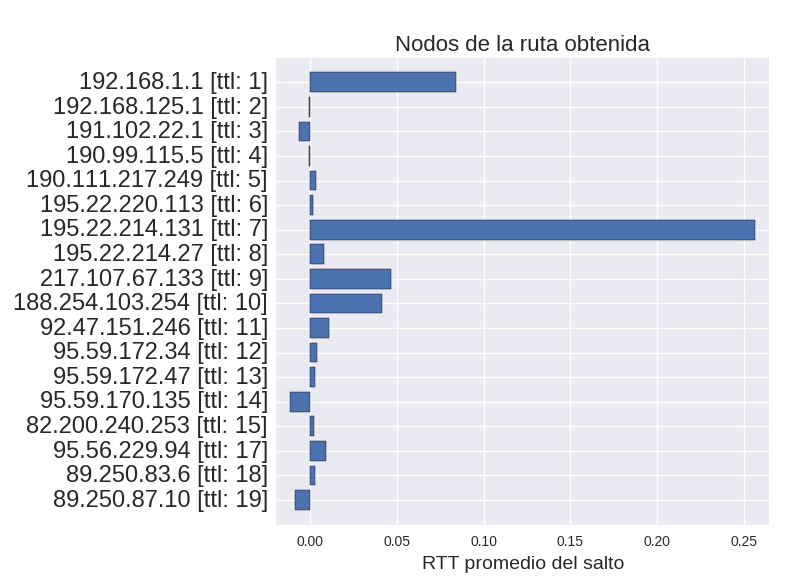
\includegraphics[width=\textwidth]{Imagenes/kazajistan_rtts.png}
  \end{subfigure}
  \label{fig:kazajthan_rtts}
  \caption{Tiempo del salto entre cada nodo y su nodo previo, para cada nodo identificado en el camino al host kaznpu.kz}
\end{figure}

\begin{figure*}[ht]
  \hspace*{-0.4cm}
  \begin{subfigure}[b]{.60\textwidth}
    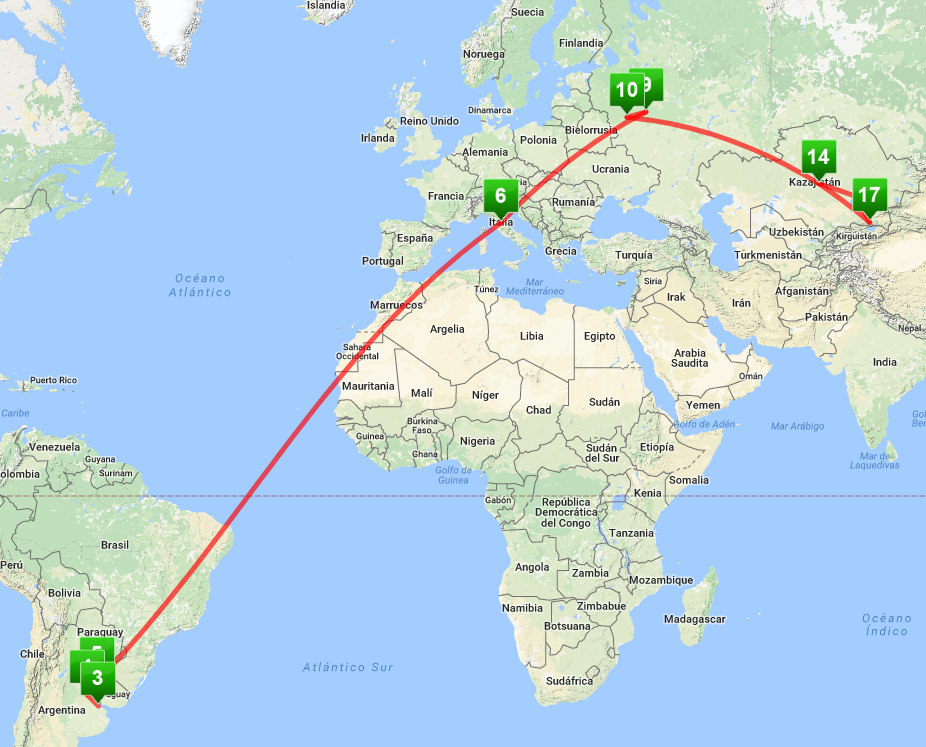
\includegraphics[width=\textwidth]{Imagenes/kazajistan_map.png}
    \label{fig:kazajthan_map}
    \caption{Mapa que muestra la unión de los nodos que forman el camino.}
  \end{subfigure}
  \begin{subfigure}[b]{.39\textwidth}
    \footnotesize
    \begin{tabular}{ l l l }
      \hline
      \textbf{TTL} & \textbf{IP} &  \textbf{País - Ciudad} \\ \hline
      1 & 192.168.1.1 &\\ \hline
      2 & 192.168.125.1 &\\ \hline
      3 & 191.102.22.1 & Argentina - Morón\\ \hline
      4 & 190.99.115.5 & Argentina - Rosario\\ \hline
      5 & 190.111.217.249 & Argentina - Entre Ríos\\ \hline
      6 & 195.22.220.113 & Italia\\ \hline
      \rowcolor[RGB]{196,214,255}
      7 & 195.22.214.131 & Italia\\ \hline
      8 & 195.22.214.27 & Italia\\ \hline
      \rowcolor[RGB]{196,214,255}
      9 & 217.107.67.133 & Rusia - Moscú \\ \hline
      \rowcolor[RGB]{196,214,255}
      10 & 188.254.103.254 & Rusia - Smolenskaya Oblast\\ \hline
      11 & 92.47.151.246 & Kazajthan\\ \hline
      12 & 95.59.172.34 & Kazajthan\\ \hline
      13 & 95.59.172.47 & Kazajthan\\ \hline
      14 & 95.59.170.135 & Kazajthan\\ \hline
      15 & 82.200.240.253 & Kazajthan\\ \hline
      17 & 95.56.229.94 & Kazajthan - Almaty Qalasy\\ \hline
      18 & 89.250.83.6 & Kazajthan\\ \hline
      19 & 89.250.87.10 & Kazajthan\\ \hline
      \hline
    \end{tabular}
    \label{fig:kazajthan_list}
    \caption{Listado de nodos: TTL, IP y ubicación geográfica.}
  \end{subfigure}
  \caption{Nodos pertenecientes al camino al host kaznpu.kz.}
\end{figure*}

\par En el gráfico de la figura 7 se observa un pico muy alto para llegar al hop cuya dirección IP es 195.22.214.131. Esto es bastante extraño porque su recorrido es local, suponemos que la causa de este comportamiento anómalo se debe a que en el hop de llegada había mucha congestión.
\par En el gráfico de la figura 9 podemos ver los 3 nodos que superan la linea del valor de Thompson. Estos son nuestros 3 outliers y candidatos a saltos intercontinentales, según nuestra herramienta. Pero como vemos en la tabla de la figura 8(b), ninguno de los 3 corresponden a saltos intercontinentales. Pero si notamos algo raro en la ruta: de \textit{Kazajthan} se redirecciona a \textit{Kazajthan - Almaty Qalasy} para luego volver a \textit{Kazajthan} inmediatamente. Notamos también que el salto de ida (hacia \textit{Almaty Qalasy}) trae aparejado un rtt un mucho mas elevado que el salto del regreso. No creemos saber por qué puede estar sucediendo esto, pero es un dato interesante que valía mencionar.

\begin{figure}[h]
  \begin{subfigure}[b]{.5\textwidth}
    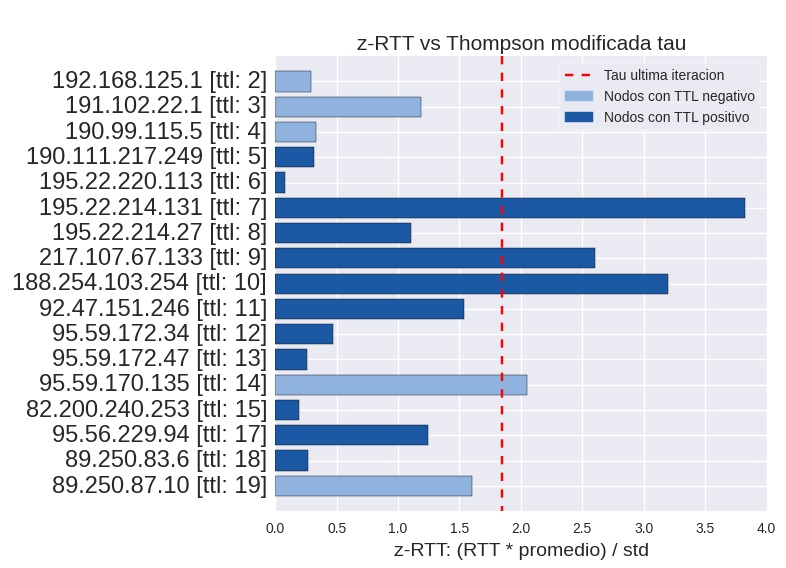
\includegraphics[width=\textwidth]{Imagenes/kazajistan_zrtts.png}
  \end{subfigure}
  \label{fig:kazajthan_zrtts}
  \caption{zRTT de los nodos del camino al host kaznpu.kz comparado con el umbral establecido por el valor de Thompson modificado.}
\end{figure}

\par Con respecto a los saltos intercontinentales, sólo hubo uno y nuestro algoritmo no logró detectarlo. A comparación de los otros experimentos la ruta final es bastante intuitiva, ya que resulta similar al camino óptimo en cuanto a recorrido (una línea recta). Al salir del país pasa por Italia, luego por Rusia y termina en la universidad de destino. Nuevamente, la mayoría de los hops respondió nuestros mensajes, lo cual permitió conocer mejor el trayecto.
